\documentclass{article}

\usepackage[utf8]{inputenc}
\usepackage[left=2cm, right=4cm, top=2cm]{geometry}
\usepackage{graphicx}
\usepackage{hyperref}
\usepackage{amsfonts}

\newcommand{\bracket}[1]{|#1\rangle}

\graphicspath{ {../../../figures/qci/} }

\title{Notes: Quantum Computation and Quantum Information: 10th Anniversary Edition}
\author{Daniel Saunders}

\begin{document}

\maketitle

\textbf{Notes}

\begin{enumerate}
	\item Some \textit{emphasis} is from the book, some is added.
	\item Abbreviations such as QC may interchangeably refer to quantum computation and quantum computer.
\end{enumerate}

\part{Fundamental concepts}

\section{Introduction and Overview}

``Information is physical'' - Rolf Landauer.

Purpose of chapter: Answer questions ``What are the fundamental concepts of quantum computation and quantum information?'', ``How can they be used?'', ``How will they be presented in the book?''.

\subsection{Global perspectives}

Quantum computation (QC) and quantum information (QI) (together, QCI): study of info. processing tasks that can be done using quantum mechanical (QM) systems.

Which fields contributed ideas to QCI? QM, computer science (CS), information theory (IT), and cryptography (crypto).

\subsubsection{History of quantum computation and quantum information}

At the turn of the 20th century, \textit{classical physics} was predicting absurdities (such as the ``\href{https://en.wikipedia.org/wiki/Ultraviolet_catastrophe}{ultraviolet catastrophe}''). These were at first resolved using additional \textit{ad hoc} hypotheses to classical physics, but became more convoluted as better understanding of atoms and radiation were obtained. In the 1920s, this crisis resulted in the creation of \textit{quantum mechanics}.

QM is a mathematical framework / set of rules for the construction of physical theories; e.g., \textit{quantum electrodynamics} (QED), which accurately describes the interaction of atoms and light.

The rules of QM are simple yet counterintuitive. One of the goals of QCI is the develop ways to sharpen our intuition about QM and make its predictions more transparent.

1980s: Is it possible to use QM effects to signal faster than light (violating Einstein's theory of relativity)? Resolution depends on whether it's possible to \textit{clone} an unknown quantum state; i.e., construct a copy of it. If cloning were possible, then it would be possible signal faster than light. However, cloning is not possible \textit{in general} in QM, due to one of the earliest results of QCI (the \href{https://en.wikipedia.org/wiki/No-cloning_theorem}{\textit{no-cloning theorem}}). Tools now exist to understand how well an imperfect quantum cloning device might work.

1970s: Interest in obtaining \textit{complete control over single quantum systems}. QM applications pre-1970s typically involved coarse-grained control over a large sample with an enormous number of QM systems, none of which were directly accessible; e.g., \href{https://en.wikipedia.org/wiki/Superconductivity}{superconductivity}. Such experiments allow for the probing of only a few aspects of QM systems, with individual system states remaining inaccessible.

Since then, several techniques for controlling single quantum states have been developed; e.g., the \href{https://en.wikipedia.org/wiki/Magnetic_trap_(atoms)}{``atom trap''} and the \href{https://en.wikipedia.org/wiki/Scanning_tunneling_microscope}{scanning tunneling microscope}.

The ability to control single QM systems is essential in order to harness QM for QCI applications.

Efforts to build quantum information processing (QIP) systems have resulted in modest success. Small quantum computers (QCs) capable of dozens of operations on a few \textit{qubits} are the state of the art (SOTA). Experimental prototypes for \textit{quantum cryptography} have also been demonstrated.

\textbf{Turning to computer science}:

\href{https://en.wikipedia.org/wiki/Alan_Turing}{Alan Turing} developed the notion of the programmable computer, a model of computation known as the \textit{Turing machine} (TM). He showed there is a \textit{Universal Turing machine} (UTM) capable of simulating any other TM. He claimed the UTM \textit{completely captures} what it means to perform an algorithmic task; i.e., if an algorithm can be performed on any hardware, there is an equivalent algorithm which does the same thing on a UTM. This is known as the \textit{Church-Turing thesis} (CT thesis) (after Alan Turing and \href{https://en.wikipedia.org/wiki/Alonzo_Church}{Alonzo Church}).

\href{https://en.wikipedia.org/wiki/John_von_Neumann}{John von Neumann} developed a theoretical model for how to assemble a digital computer as capable as a UTM. \textit{Moore's law} refers to the tendency of computer power to roughly double for constant cost every two years, coined by \href{https://en.wikipedia.org/wiki/Gordon_Moore}{Gordon Moore} in 1965.

Moore's law has held approximately since its inception, but this is expected to end since conventional approaches to microchip fabrication are starting to run up against fundamental size difficulties; i.e., quantum effects are interfering in the functioning of electronic devices as they're made increasingly smaller.

One solution to this problem: move to a different computing paradigm, one of which is provided by QC. Although classical computers (CCs) can simulate QC, it appears impossible to do so \textit{efficiently}, resulting in a QC speed advantage over DC. Researchers believe that \textit{no} amount of progress in CC is enough to overcome this advantage.

Key notions of ``efficiency'' in computer algorithms is made mathematically precise by \textit{computational complexity}; roughly, efficient algorithms run in polynomial time in the size of the problem solved, whereas inefficient algorithms require super-polynomial time. In the 1960s-70s, it seemed that the TM model of computation (MoC) was at least as powerful as any other MoC, in that any problem efficiently solved by another MoC could be efficiently solved by the TM model by using the TM to simulate the other MoC. This results in the \textit{strong CT} thesis: \textit{Any algorithmic process can be simulated efficiently using a Turing machine}.

Researchers in the field of \textit{analog computation} (AC) noticed that certain type of ACs can efficiently solve problems without known efficient TM solutions. However, when realistic assumptions about presence of noise in ACs is used, their power disappars: they can't efficiently solve problems than TMs can't. The development of \textit{quantum error-correcting codes} and \textit{fault-tolerant quantum computation} solved this problem for QCI. Unlike AC, QC can tolerate a finite amount of noise and still retain a computational advantage.

First major challenge to strong CT thesis (1970s): Solovay and Strassesn showed that it's possible to test for primality using a \textit{randomized algorithm}. It could determine that a number was \textit{probably} prime or otherwise composite \textit{with certainty}. The test could be repeated to improve confidence in the results of the probabilistic test. It seemed that computers with a random number generator (RNG) could efficiently solve problems with no efficient solution on deterministic TMs.

Randomized algorithms pose a challenge to the strong CT thesis, resulting in another modification of the strong CT thesis: \textit{Any algorithmic process can be simulated efficiently using a probabilistic Turing machine}.

1985: \href{https://en.wikipedia.org/wiki/David_Deutsch}{David Deutsch} asked whether the laws of physics could be used to derive a stronger CT thesis, instead of using \textit{ad hoc} hypothesis. He attempted to device a version of a TM that would be capable simulating an \textit{arbitrary} physical system, and, since the laws of physics are quantum mechanical, was led to consider computing devices based on QM principles.

It's not clear wther the quantum TM (QTM) is sufficient to efficiently simulate an arbitrary physical system. It's possible that some effect of more complicated physical theories may be required to enable still more powerful computation.

The QTM posed another challenge to the strong, probabilistic CT thesis. Deutsch constructed an example suggesting that QCs might have computational power exceeding those of CCs; i.e., that QCs can efficiently solve problems which have no efficient solution on classical computers.

This first step was improved in the next decade, culminating with Peter Shor's algorithm(s) for the efficient QC solution of the prime factorization and ``discrete logarithm'' problems (1994). These problems are still believed not to have efficient solutions on CCs. Lev Grover demonstrated a QC speedup on search in unstructured search spaces (1995).

1982: Richard Feynman pointed out the seemingly essential difficulties in simulating QM systems with CCs, and suggeseting QCs would avoid these. 1990s: A team of researchers showed it is indeed possible to efficiently simulate QM systems with no known efficient simulation on CCs. Likely major application of QCs: perfoming simulations of such QM systems.

Designing quantum algorithms (QAs) seems to be hard, perhaps because designers face two problems not faced in algorithm design for CCs:

\begin{enumerate}
\item Human intuition is apparently rooted in the ``classical world''. To design good QAs, one must ignore classical intuition for at least part of the design process and use quantum effects to achieve the algorithmic goal.
\item The QA much be better than any existing classical algorithm. Although a QA may make use of aspects of QM, it may not be of interest as a classical algorithm (CA) with similar performance characteristics may exist.
\end{enumerate}

What is is that makes QCs more powerful than CCs? What class of problems can be solved efficiently on QCs, and how does that compare to the same class of problems for CCs?

\textbf{Turning to information theory}:

1948: \href{https://en.wikipedia.org/wiki/Claude_Shannon}{Claude Shannon} published a pair of papers on the foundations of the theory of information and communication. Key step: \textit{mathematically defining hte concept of information}. Two key questions relation to communication of information over a channel:

\begin{enumerate}
\item What resources are needed to send information over a channel?
\item Can information be transmitted such that it's protected against noise in the channel?
\end{enumerate}

Shannon answered these questions with two fundamental IT theorems:

\begin{enumerate}
\item The \textit{noiseless channel coding theorem} quantifies the physical resources needed to store the output from an information source.
\item The \textit{noisy channel coding theorem} quantifies how much information it's possible to reliably transmit through a noisy channel. To get reliable transmission in the presence of noise, \textit{error-correcting codes} (ECCs) could be used to protect the information being sent. This theorem gives an upper limit on the protection afforded by ECCs.
\end{enumerate}

A sophisticated theory of ECCs now exists.

Quantum information theory (QIT) follows a similar developments. 1995: \href{https://en.wikipedia.org/wiki/Benjamin_Schumacher}{Ben Schumacher} provided an another of the noiseless channel coding theorem and defined the \textit{quantum bit}, or \textit{qubit}, as the tangible physical resource. No analogue to the noisy channel coding theorem is known for QIT. A theory of quantum EC (QEC) has been developed, allowing QCs to compute effectively in the presence of noise, and allows reliable communcation over noisy quantum channels.

1992: Charles Bennett and Stephen Wiesner showed how to transmit two classical bits of information while only transmitting one quantum bit; called \textit{superdense coding}.

\textit{Distributed quantum computation}: exponentially less communication is sometimes required to solve problems with networked QCs than with networked CCs.

\textit{Networked information theory}: The study of networks of multiple communications channels.

Study of networked QIT is in its infancy; no unifying theory of networked IT exists for QCs. 

\textbf{Turning to cryptography}:

Cryptography is the problem of doing communication or computation with two or more parties who many not trust each other. Secret communication can be accomplished using a \textit{cryptographic protocol}, distinguishing between \textit{private key} and \textit{public key cryptosystems}.

\textit{Quantum cryptography} or \textit{quantum key distribution} allows for private crypto key distribution such that Alice and Bob's security cannot be compromised. Basic idea: exploit QM principle that observations disturbs QM systems. Eavesdroppers can be detected as a disturbance of the communication channel Alice and Bob use to establish a private key. 1984: Charles Bennet and Gilles Brassard proposed a QM protocol to distribute keys between Alice and Bob without possibility of compromise.

\textit{Public key cryptosystems}: Bob publishes a ``public key'' which Alice uses to encrypt a message to Bob, which is extremely difficult to decrypt without the private key known only to Bob. Such cryptosystems solve the key distribution problem by making it unnecessary to share private keys before communication.

Presumed security of the \textit{RSA cryptosystem} relies on the belief that factoring is hard to solve using CCs. Shor's algorithm for factoring on QCs could break RSA!

\textit{Quantum entanglement}: uniquely QM \textit{resource} that plays a role in many interesting applications of QCI; not well understood.

\subsubsection{Future directions}

QCI has taught us to \textit{think physically about computation}; any physical theory may be used as the basis for a theory of information processing and communication. On the other hand, we may also \textit{think computationally about physics}. Physics has traditionally focused on understanding elementary objects and simple systems; computation and algorithms provide means for constructing and understanding complex systems.

\subsection{Quantum bits}

QCI are built on a concept analogous the to classical \textit{bit}, the \textit{qubit} or \textit{quantum bit}. They have a physical realization, but will be described as \textit{mathematical objects} with certain properties, since treating them as abstract entities gives the freedom to construct a general theory of QCI which doesn't depend on a specific physical system for realization.

A qubit has a \textit{state}, just like a bit. Two possible states are $\bracket{0}$ and $\bracket{1}$, corresponding to the 0 and 1 states for classical bits. This is called the \textit{Dirac notation}. It's possible to form \textit{linear combinations} of states, often called \textit{superpositions}:

\begin{equation} \label{eq:1}
\bracket{\psi} = \alpha \bracket{0} + \beta \bracket{1}.
\end{equation}

The numbers $\alpha$ and $\beta$ are complex numbers, and the state of a qubit is a vector in a two-dimensional complex vector space. The special states $\bracket{0}$ and $\bracket{1}$ are called \textit{computational basis states} and form an orthonormal basis for the vector space.

We can't examine a qubit to determine its quantum state (the values of $\alpha$ and $\beta$). We can acquire more restricted information by measuring a qubit a obtaining a 0 with probability $|\alpha|^2$ or a 1 with probability $|\beta|^2$. Thus, a qubit's state is a unit vector in a two-dimensional complex vector space.

There is an indirect correspondence between qubit states and their consequences, and they can be manipulated and transformed in ways that lead to measurement outcomes that depend on their properties.

Classical bits are like coins: they can exist either in a heads up (1) or tails up (1) state. Qubits, OTOH, can exist in a \textit{continuum} of states between $\bracket{0}$ and $\bracket{1}$, but only ever gives ``0'' or ``1' (probabilistic) outcomes when measured. A qubit can be in the state (denoted $\bracket{+}$)

\begin{equation} \label{eq:2}
\frac{1}{\sqrt{2}} \bracket{0} + \frac{1}{\sqrt{2}} \bracket{1},
\end{equation}

which gives 0 or 1 each with probability $\frac{1}{2}$.

Because $|\alpha|^2 + |\beta|^2 = 1$, we can rewrite Equation \ref{eq:1} as

\begin{equation} \label{eq:3}
\bracket{\psi} = e^{i \gamma} \left(\cos \frac{\theta}{2} \bracket{0} + e^{i \varphi} \sin \frac{\theta}{2} \bracket{1} \right)
\end{equation}

where $\theta, \varphi, \gamma \in \mathbb{R}$. We will later see that we can \textit{ignore} the factor in front because it has \textit{no observable effects} and effectively write

\begin{equation} \label{eq:4}
\bracket{\phi} = \cos \frac{\theta}{2} \bracket{0} + e^{i \varphi} \sin \frac{\theta}{2} \bracket{1}
\end{equation}

The numbers $\theta$ and $\varphi$ define a point on the unit 3D sphre, called the \textit{Bloch sphere}, useful for visualizing state of a single qubit (Figure \ref{fig:1}).

\begin{figure} \label{fig:1}
	\centering
	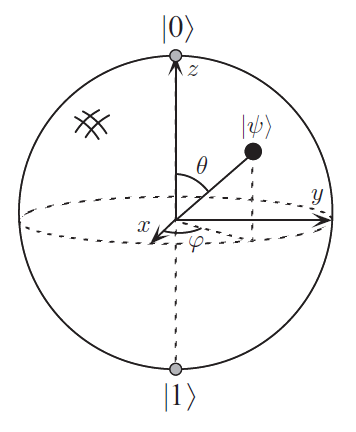
\includegraphics[width=0.5\textwidth]{bloch_sphere.png}
	\caption{Bloch sphere representation of a qubit.}
\end{figure}

\end{document}
